\chapter{Convexity}

Our goal in this lecture is to solve problems of the form 
\begin{equation}
    \min_{x\in C} f(x)
\end{equation}
where $C\subset V$ is a \emph{convex subset} of the space $V$ and $f:C\rightarrow (-\infty,\infty]$ is a \emph{convex function}. Therefore, in the following we will analyze in more detail what convexity of sets and functions precisely means and what consequences we can draw from those properties.

\section{Convex sets}
A set is called convex if for any two points within the set, the entire straight line connecting the points as contained in the set as well. More formally:
\begin{defn}
    A set $C\subset V$ is called convex iff for every $x,y\in C$, $\lambda\in (0,1)$ it holds
    \begin{equation}
        \lambda x + (1-\lambda) y\in C.
    \end{equation}
\end{defn}

Note that
\begin{equation}
    \lambda x + (1-\lambda) y = y + \lambda(x-y)
\end{equation}
which shows more clearly that $\lambda x + (1-\lambda) y$ is the line connecting $x$ and $y$.

Moreover, we can easily show the following using more general \emph{convex combinations}.

\begin{lemma}
    The set $C\subset V$ is convex if and only if for every $n\in \N$, $x_i\in C$, $\lambda_i\in [0,1]$, $i=1,\dots,n$ with $\sum_{i=1}^n\lambda_i=1$ it holds
    \begin{equation}
        \sum_{i=1}^n\lambda_i x_i \in C.
    \end{equation}
\end{lemma}
\begin{proof}
    Exercise.
\end{proof}

For notational convenience we define the \emph{unit simplex} as 
\begin{equation}
    \Delta^k = \{(\lambda_1,\dots,\lambda_k)\in [0,1]\;|\;\sum_{i=1}^n\lambda_i = 1\}
\end{equation}
We may now define the smalles convex set containing a given set, the \emph{convex hull}.

\begin{defn}[Convex hull]
    Let $C\subset V$. The convex hull of $C$ is defined as the set
    \begin{equation}\label{eq:convex_sets:defin_conv_hull}
        \conv(C) \coloneqq \bigcap_{\substack{S\subset V \text{ convex}\\C\subset S}}S
    \end{equation}
\end{defn}

\begin{lemma}
    It holds true that
    \begin{equation}\label{eq:convex_sets:conv_hull}
        \conv(C) = \bigg\{ \sum_{i=1}^n\lambda_i x_i\;|\; n\in \N,\;x_i\in C, \; \lambda\in \Delta^n\bigg\}
    \end{equation}
\end{lemma}
\begin{proof}
    Let us denote the right-hand side of \eqref{eq:convex_sets:conv_hull} as $A$.
    We will show that $\conv(C)\subset A$ and $A\subset\conv (C)$.

    \underline{$A\subset\conv (C)$:}
    Let $x=\sum_{i=1}^n\lambda_i x_i\in A$. Note that for any $S\subset V$ such that $S$ is convex and $C\subset S$ it holds that $x\in S$. Therefore, $x\in \conv(C)$ by its definition in~\eqref{eq:convex_sets:defin_conv_hull}.

    \underline{$\conv (C)\subset A$:} 
    One may easily check that $A$ is, indeed, a convex set. Moreover $C\subset A$. Therefore, $A$ appears as one of the sets $S$ in~\eqref{eq:convex_sets:defin_conv_hull} and, thus, $\conv(C)\subset A$.
\end{proof}


\begin{figure}
    \centering
    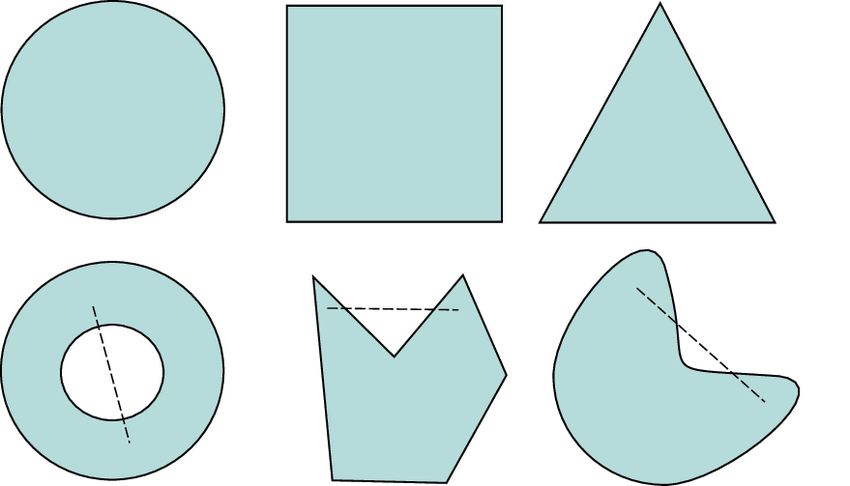
\includegraphics[width=.7\textwidth]{figures/sets.png}
    \caption{Top row: convex sets. Bottom row: non-convex sets.}
\end{figure}

\begin{example}
    The following are convex sets (the proofs are left as exercises):
    \begin{itemize}
        \item The empty set $\emptyset$
        \item Every vector space
        \item Every norm ball, that is, for every norm $\|\emptyarg\|$ and every $c\in V$ and $R\geq 0$ the sets
        \begin{equation}
            B_{\|\emptyarg\|,R}(c)\{x\in V\;|\; \|x-c\|< R\}
        \end{equation}
        and
        \begin{equation}
            \overline{B}_{\|\emptyarg\|,R}(c)\{x\in V\;|\; \|x-c\|\leq R\}
        \end{equation}
        \item Every affine subspace, that is, for any set of vectors $z, x_1,\dots,x_k\in V$ the set
        \begin{equation}
            \bigg\{ x\in V\;|\; x = z + \sum_{i=1}^k\lambda_i x_i,\; \lambda_i\in \R \bigg\}
        \end{equation}
    \end{itemize}
\end{example}

\begin{figure}
    \centering
	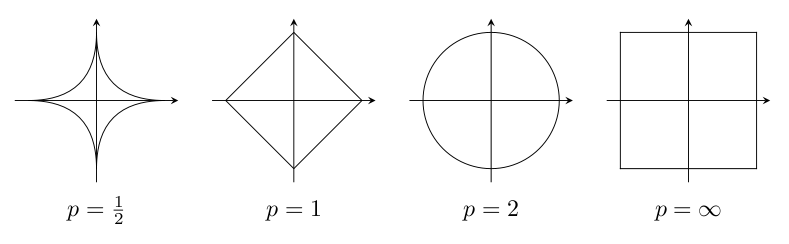
\includegraphics[width=1\textwidth]{figures/balls.png}
    \caption{Norm balls for $\overline{B}_{\|\emptyarg\|_p,R}(0)$ for different $\ell^p$ norms. Note that the set is not convex for $p=1/2$ as this choise does not lead to a norm (no triangle inequality).}
\end{figure}

\begin{lemma}[Operations that preserve convexity]\label{convexity:lemma:ops preserving convexity}
    The following hold true:
    \begin{enumerate}
        \item Intersection. Let $C_i\subset V$ be convex for $i\in I$ with $I$ an arbitrary index set. Then the intersection
        \begin{equation}
            \bigcap_{i\in I} C_i \coloneqq \{x\in V\;|\; x\in C_i\; \forall i\in I\}
        \end{equation}
        is convex.
        \item Weighted sum. Let $C_i\subset V$ be convex for $i=1,\dots, N$. Moreover let $\lambda_i \in \R$ for $i=1,\dots, N$. Then the set
        \begin{equation}
            \sum_{i=1}^n \lambda_i C_i \coloneqq \bigg\{\sum_{i=1}^N \lambda_i x_i\;|\; x_i\in C_i\; \forall i\in I\bigg\}
        \end{equation}
        is convex.
        \item Cartesian product sum. Let $C_i\subset V$ be convex for $i\in I$ with $I$ an arbitrary index set. Then the cartesian product
        \begin{equation}
            \bigotimes_{i\in I} C_i \coloneqq \{(x_i)_{i\in I}\;|\; x_i\in C_i\; \forall i\in I\}
        \end{equation}
        is convex.
        \item Images and preimages\footnote{The preimage is well-defined also for non-invertible maps!} of linear maps are convex, that is, for $A:V\rightarrow W$ linear and $S\subset V$, $T\subset W$ both convex the following sets are convex:
        \begin{equation}
            A(S) = \{Ax \;|\; x\in S\},\quad A^{-1}= \{y\in V\;|\; Ax \in T\}
        \end{equation}
    \end{enumerate}
\end{lemma}
\begin{proof}
    We only prove the first part and leave the remainder as an exercise. The proof is straight-forward. Let $x,y\in \bigcap_{i\in I} C_i$ and $\lambda\in (0,1)$. Since $x,y\in C_i$ for every $i$ and each $C_i$ is convex, it follows that $\lambda x + (1-\lambda)y \in C_i$ for every $i$ and, therefore, $\lambda x + (1-\lambda)y \in \bigcap_{i\in I} C_i$.
\end{proof}

We want to formally define the notion of a hyperplane, that is, the generalization to arbitrary dimensions of a 2D plane in $\R^3$.

\begin{defn}[Hyperplanes]
    Let $V$ be an inner product space, a hpyerplane is a set $H$ of the form
    \begin{equation}
        H = \{x\in V\;|\; \inner{x}{a}=b\}
    \end{equation}
    for some $a\in V\setminus\{0\}$, $b\in\R$.
\end{defn}

The parameter $a$ defines the angle of the plane and $b$ its offset. In particular, for $0\in H$ iff $b=0$ in which case $H$ is a subspace. Whenever $b\neq 0$, $H$ is merely an affine subspace.

Note that if $x_0\in H$ it holds that
\begin{equation}
    H = \{x\in V\;|\; \inner{x-x_0}{a}=0\}.
\end{equation}
It follows that $a$ is the normal vector to the plane. Moreover one can check (exercise) that $\frac{|b|}{\|a\|}$ is the distance of the plane from the origin.

Note that every hyperplane separates the space into two halfs. 
\begin{defn}[Halfspaces]
    Let $V$ be an inner product space, a halfspace is a set $H^-$ of the form
    \begin{equation}
        H^- = \{x\in V\;|\; \inner{x}{a}\leq b\}
    \end{equation}
    for some $a\in V\setminus\{0\}$, $b\in\R$.
\end{defn}

The following theorem, which states that this separation can be chosen in a particular manner, is in fact surprisingly crucial within optimization and functional analysis!

\begin{theorem}[Hahn-Banach seperation theorem]
    Let $S,T$ be two nonempty, disjoint, convex subsets of a vector space $V$ with $S$ open. Then there exists $a\in V^*$, $a\neq 0$ and $\alpha\in \R$ such that
    \begin{equation}
        \inner{x}{a}<\inner{y}{a},\quad x\in S, \; y\in T.
    \end{equation}
    If $S,T$ are both closed and one of them is compact, there exists $\alpha\in \R$ and $\epsilon>0$ such that 
    \begin{equation}
        \inner{x}{a}\leq \alpha\leq \alpha+\epsilon\leq \inner{y}{a},\quad x\in S, \; y\in T.
    \end{equation}
\end{theorem}
The second version allows to find a strictly positive difference between 
\[
    \sup_{x\in S}\inner{x}{a}
    \quad 
    \text{and}
    \quad
    \inf_{y\in T}\inner{y}{a}.
\]

\begin{figure}
    \centering
			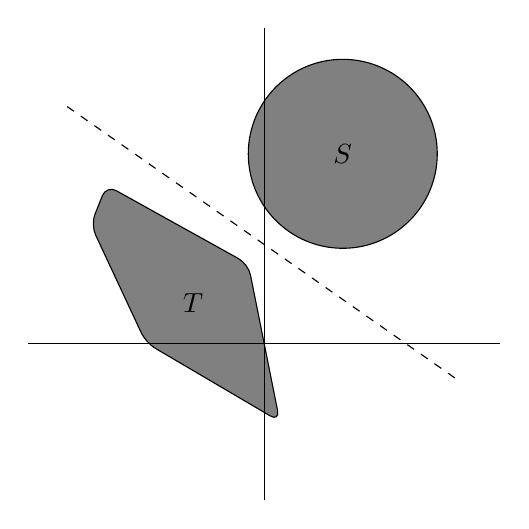
\begin{tikzpicture}[font=\sffamily]
				\draw[dashed] (-2.5,3) -- (2.5,-0.5);
				\node[circle,draw,fill=gray,minimum size=2.4cm] at (1,2.4) {$S$};
				\draw[fill=gray,rounded corners] (-2,2) -- (-0.2,1) -- (0.2,-1) -- (-1.5,0) -- (-2.2,1.5) --cycle;
				\path (-2,2) --  (0.2,-1)  node[midway] {$T$};
				\draw[ultra thin] (-3,0) -- (3,0) (0,-2) -- (0,4);
			\end{tikzpicture}\hfill%
			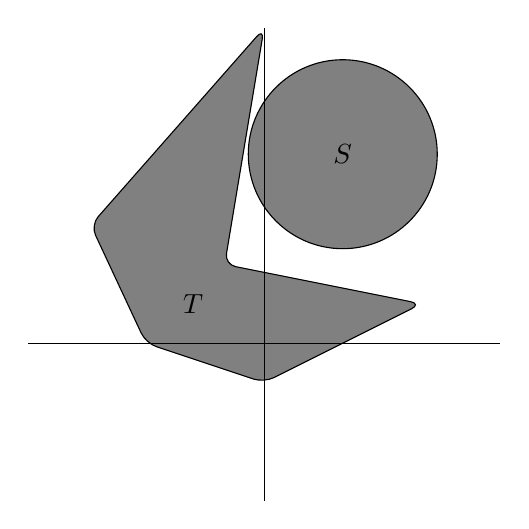
\begin{tikzpicture}[font=\sffamily]
				\node[circle,draw,fill=gray,minimum size=2.4cm] at (1,2.4) {$S$};
				\draw[fill=gray,rounded corners] (0,4) -- (-0.5,1) -- (.5,.8) -- (2,.5) -- (0,-.5) -- (-1.5,0) -- (-2.2,1.5) --cycle;
				\path (-2,2) --  (0.2,-1)  node[midway] {$T$};
				\draw[ultra thin] (-3,0) -- (3,0) (0,-2) -- (0,4);
			\end{tikzpicture}
    \caption{Illustration of the Hahn-Banach seperation theorem and why it may fail without convexity.}
\end{figure}

\section{Convex functions}
As shown in~\cref{fig:convexity:1d_example} convexity has crucial impacts on the questions of existence and uniqueness of minima.
\begin{figure}
    \centering
    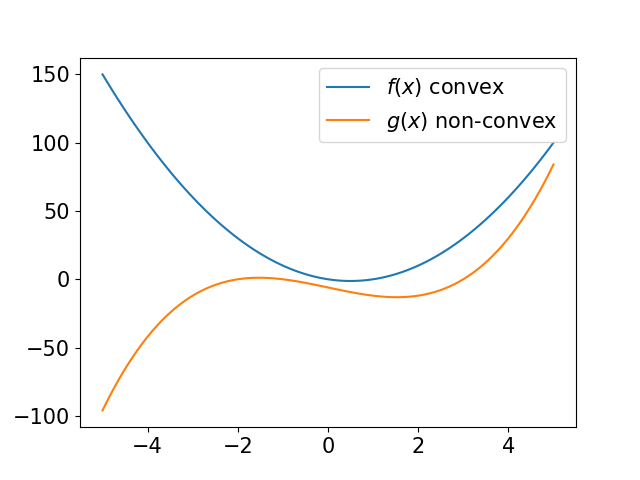
\includegraphics[width=0.5\textwidth]{figures/convex_fct.png}
    \caption{Example of a convex vs a non-convex function in 1D.}
    \label{fig:convexity:1d_example}
\end{figure}

\begin{defn}[Zero-order condition for convexity]
    Let $C\subset V$ be convex and $f:C\rightarrow (-\infty,\infty]$.
    \begin{itemize}
        \item We call $f$ convex iff for any $x,y\in C$ and $\lambda\in (0,1)$ it holds
        \begin{equation}
            f(\lambda x + (1-\lambda)y)\leq \lambda f( x ) + (1-\lambda)f(y).
        \end{equation}
        \item We call $f$ strictly convex iff for any $x,y\in C$ and $\lambda\in (0,1)$ it holds
        \begin{equation}
            f(\lambda x + (1-\lambda)y) < \lambda f( x ) + (1-\lambda)f(y).
        \end{equation}
        \item We call $f$ $\mu$-strongly convex iff for any $x,y\in C$ and $\lambda\in (0,1)$ it holds
        \begin{equation}
            f(\lambda x + (1-\lambda)y) \leq \lambda f( x ) + (1-\lambda)f(y) - \frac{\lambda(1-\lambda)\mu}{2}\|x-y\|^2
        \end{equation}
    \end{itemize}
\end{defn}
The zero-order condition states that the straight line connecting to points on the graph (the secant) is always above the function. In the case of a strictly convex function the secant is strictly above the function and in the strongly convex case we may even \emph{squeeze} a quadratic inbetween.


\begin{figure}
    \centering
    \begin{tikzpicture}[inner sep=.5mm,
			declare function={
				f(\x)= (\x-3)^2+3*\x-4;
			}
			]
			\begin{axis}[axis lines=middle,domain=-1:4,samples=200,xtick={0.5,3},xticklabels={$x$,$y$},ytick=\empty,xmin=-.2,xmax=3.7,ymin=-.1,ymax=10]
				\addplot[blue,very thick,name path=f] {f(x)};
				\pgfplotsinvokeforeach{.5,3}{
					\path[name path=x] (#1,0) -- (#1,6);
					\draw[black!50,thick,dashed,name intersections={of=f and x, name=i}] (#1,0) -- (i-1);
				}
				\draw[very thick] ($(.5,{f(.5)})$) node[circle,fill=blue,label=left:{$f(x)$}]{} -- ($(3,{f(3)})$) node[circle,fill=blue,label=right:{$f(y)$}]{};
				\node[text=blue] at (1.75,2) {$f(\lambda x+(1-\lambda)y)$};
				\node[rotate=10] at (1.75,5) {$\lambda f(x)+(1-\lambda)f(y)$};
			\end{axis}
		\end{tikzpicture}
        \caption{Geometric interpretation of the zero-order condition for convexity of a function.}
\end{figure}


\begin{example}
    The following are convex (proof: exercise):
    \begin{enumerate}
        \item Affine functions $f(x)=\langle y, x\rangle + b$ with $a\in V$, $b\in \R$ (in particular, linear functions for $b=0$).
        \item All norms are convex functions.
    \end{enumerate}
\end{example}

Similar to the corresponding result for convex sets we can extend convexity to arbitrarily \emph{large} convex combinations.

\begin{theorem}[Jensen]
    Let $C\subset V$ be convex and $f:C\rightarrow \bR$. Then $f$ is convex iff for any $k\in \N$, $\lambda\in \Delta^k$, and $x_i\in C$ it holds
    \begin{equation}
        f(\sum_{i=1}^k\lambda_i x_i)\leq \sum_{i=1}^k\lambda_i f(x_i)
    \end{equation}
\end{theorem}

We have seen above that convexity means that the secant stays above the function. It also means, that the tangent stays below the function (\cf~\cref{convexity:fig:gradients}). 

\begin{theorem}[First-order characterization of convexity]\label{convexity:thm:first_order}
    Let $f:C\rightarrow\R$ continuously differentiable with $C\subset\R^d$ convex.
    \begin{itemize}
        \item $f$ is convex iff for all $x,y\in C$
        \[
            f(x) + \langle \nabla f(x),y-x\rangle \leq f(y).
        \]
        \item $f$ is strictly convex iff the above inequality holds strict for all $x\neq y$.
    \end{itemize}
\end{theorem}
\begin{proof}
    We only show the first item as the second follows trivially.
    
    $\Rightarrow$: Let $f$ be convex. then we have
    \begin{equation}
        f(x+\lambda (y-x)) = f(\lambda y + (1-\lambda)x)\leq \lambda f(y) + (1-\lambda) f(x).
    \end{equation}
    Rearranging yields
    \begin{equation}
        \frac{f(x+\lambda (y-x))-f(x)}{\lambda} \leq f(y) - f(x).
    \end{equation}
    Letting $\lambda\rightarrow 0$ yields the result.

    $\Leftarrow$: Assume now the gradient condition holds true. Let us denote $x_\lambda = x+\lambda (y-x)$
    \begin{equation*}
        f(x_\lambda) + \langle \nabla f(x_\lambda), y-x_\lambda\rangle = f(x_\lambda) + \langle \nabla f(x_\lambda), (1-\lambda) (y-x)\rangle \leq f(y)
    \end{equation*}
    and
    \begin{equation*}
        f(x_\lambda) + \langle \nabla f(x_\lambda), x-x_\lambda\rangle = f(x_\lambda) + \langle \nabla f(x_\lambda), -\lambda(y-x)\rangle \leq f(x).
    \end{equation*}
    Multiplying the first inequality with $\lambda$, the second with $1-\lambda$ and adding both leads to
    \begin{equation*}
        f(x_\lambda) \leq \lambda f(y) +(1-\lambda) f(x).
    \end{equation*}
\end{proof}


\begin{figure}
    \centering
    \begin{tikzpicture}[inner sep=.5mm,
			declare function={
				f(\x)=  (\x-3)^2+3*\x-4;
			}
			]
			\begin{axis}[axis lines=middle,domain=-1:4,samples=200,xtick={2},xticklabels={$x$},ytick=\empty,xmin=-.2,xmax=3.7,ymin=-.1,ymax=10]
				\addplot[blue,very thick,name path=f] {f(x)};
				\pgfplotsinvokeforeach{2}{
					\path[name path=x] (#1,0) -- (#1,6);
					\draw[black!50,thick,dashed,name intersections={of=f and x, name=i}] (#1,0) -- (i-1);
				}
				\addplot[very thick] {f(2)+1*(x-2)};
				\node[circle,fill=blue,label=above:{$f(x)$}] at ($(2,{f(2)})$) {};
				\node[text=blue,yshift=5mm] at ($(.5,{f(.5)})$) {$f$};
			\end{axis}
			\node[rotate=17,yshift=-3mm] at (6, 2.5) {$\textcolor{black}{y \mapsto f(x)+\inner{\nabla f(x)}{y-x}}$};
		\end{tikzpicture}
        \caption{Geometric interpretation of a convex function.}
        \label{convexity:fig:gradients}
\end{figure}

\begin{defn}[Minimum]
    Let $f:C\rightarrow \R$. 
    \begin{itemize}
        \item We call $x^*$ a local minimum iff there exists $\epsilon>0$ such that 
        \[
            f(x^*)\leq f(x),\quad \forall x\in B_\epsilon(x^*)
        \]
        \item We call $x^*$ a global minimum iff
        \[
            f(x^*)\leq f(x),\quad \forall x\in C
        \]
    \end{itemize}
    The minimum is called \emph{strict} if the above inequalities hold strict.
\end{defn}

We are now in the position to prove a first crucial result of convex optimization.
\begin{prop}\label{convexity:prop:OC1}
    Let $f:C\rightarrow \R$ continuously differentiable over a convex set. If $\nabla f(x^*)=0$ then $x^*$ is a \textbf{global} minimizer.
\end{prop}
\begin{proof}
    By the first-order characterization of convexity we have
    \begin{equation}
        f(x)\geq f(x^*) + \langle \nabla f(x^*),x-x^*\rangle
        = f(x^*) + 0.
    \end{equation}
\end{proof}

Note, that the converse of~\cref{convexity:prop:OC1}, that is, the implication
\begin{equation}
    \text{$x^*$ is minimum} \Rightarrow \nabla f(x^*) = 0
\end{equation}
is in general only true if $x^*$ is contained in the interior of $C$ denoted as $C^\circ$, that is, there exists $\epsilon>0$ such that $B_\epsilon(x^*)\subset C$.

\begin{theorem}
    Let $f:C\rightarrow \R$ continuously differentiable over a convex set and $x^*\in C^\circ$. Then $\nabla f(x^*)=0$ iff $x^*$ is a global minimizer.
\end{theorem}
\begin{proof}
    One direction follows from~\cref{convexity:prop:OC1}. For the other direction, assume that $x^*$ is a minimum. Therefore, for any $v\in\R^d$, if $t>0$ is sufficiently small, it follows by optimality
    \begin{equation}
        f(x^*+tv) - f(x^*)\geq 0.
    \end{equation}
    Dividing by $t$, since $t>0$ yields
    \begin{equation}
        \frac{f(x^*+tv) - f(x^*)}{t}\geq 0.
    \end{equation}
    Letting $t\rightarrow 0$ yields 
    \begin{equation}
        \langle\nabla f(x^*), v\rangle\geq 0.
    \end{equation}
    Since $v$ was arbitrary, we may repate the same argument with $-v$ leading to $\langle\nabla f(x^*), v\rangle\leq 0$ and, therefore, in total to $\langle\nabla f(x^*), v\rangle = 0$. Again, since $v$ was arbitrary, we have $\nabla f(x^*)=0$ (why?).
\end{proof}

You may remember that in 1D, if the function is differentiable., convexity can be characterized by monotonicity of the derivative. In arbitrary dimensions we have the following result.

\begin{theorem}[Monotonicity of the gradient]
    Let $f:C\rightarrow\R$ be continuously differentiable over a convex set $C$. Then $f$ is convex iff
    \begin{equation}
        \langle\nabla f(x) - \nabla f(y),x-y\rangle\geq 0.
    \end{equation}
\end{theorem}
\begin{proof}
    $\Rightarrow$: Assume $f$ is convex. By the first-order characterization of convexity we have 
    \begin{equation}
        \begin{aligned}
            &f(x) + \langle\nabla f(x), y-x\rangle\leq f(y),\\
            &f(y) + \langle\nabla f(y), x-y\rangle\leq f(x).
        \end{aligned}
    \end{equation}
    Adding both equation yields the result.

    $\Leftarrow$: Assume $\nabla f$ is monotone. By the fundamental theorem of calculus we have
    \begin{equation}
        \begin{aligned}
            f(y) - f(x) 
            &= \int_0^1 \frac{\dd}{\dd t}f(x+t(y-x))\dd t\\
            &= \int_0^1 \langle\nabla f(x+t(y-x)), y-x\rangle\dd t\\
            &= \int_0^1 \langle\nabla f(x+t(y-x))-\nabla f(x), y-x\rangle\dd t + \langle\nabla f(x), y-x\rangle\\
            &= \int_0^1 \frac{1}{t}\underbrace{\langle\nabla f(x+t(y-x))-\nabla f(x), t(y-x)\rangle}_{\geq 0}\dd t + \langle \nabla f(x), y-x\rangle\\
            &\geq \langle \nabla f(x), y-x\rangle
        \end{aligned}
    \end{equation}
\end{proof}

Finally, we can also use the second derivative to characterize convexity. Intuitivelly, convexity means \emph{positive curvature}. To formalize this, we recall, how matrices are \emph{ordered}. For two matrices $A,B\in \R^{d\times d}$ we write
\begin{equation}
    A\succeq B \Longleftrightarrow \langle x, A x\rangle \geq \langle x, B x\rangle,\; \forall x\in\R^d
\end{equation}
and, similarly,
\begin{equation}
    A\succ B \Longleftrightarrow \langle x, A x\rangle > \langle x, B x\rangle,\; \forall x\in\R^d.
\end{equation}

\begin{theorem}[Second order characterization of convexity]
    Let $f:C\rightarrow \R$ be twice continuously differentiable over a convex set $C$. 
    \begin{enumerate}
        \item $f$ is convex iff $\nabla^2 f(x)\succeq 0$.
        \item $f$ is strictly convex iff $\nabla^2 f(x)\succ 0$.
    \end{enumerate}
\end{theorem}
\begin{proof}
    We only proof the first assertion.

    $\Rightarrow$: Assume $f$ is convex. By monotonicity of the gradient it follows for $t>0$
    \begin{equation}
        \frac{\inner{\nabla f(x+tv)-\nabla f(x)}{v}}{t}\geq 0.
    \end{equation}
    Letting $t\rightarrow 0$ it follows 
    \begin{equation}
        \langle v, \nabla^2 f(x)v\rangle\geq 0.
    \end{equation}
    Since $v$ was arbitrary, the result follows.

    $\Leftarrow$: Assume $\nabla^2 f\succeq 0$. By the fundamental theorem of calculus we have
    \begin{equation}
        \begin{aligned}
            \nabla f(y) - \nabla f(x)
            =& \int_0^1 \frac{\dd}{\dd t} \nabla f(x+t(y-x))\dd t\\
            =& \int_0^1 \nabla^2 f(x+t(y-x))(y-x)\dd t.
        \end{aligned}
    \end{equation}
    Multiplying by $y-x$ yields
    \begin{equation}
        \begin{aligned}
            \langle \nabla f(y) - \nabla f(x),y-x\rangle
            =& \int_0^1 \frac{\dd}{\dd t} \nabla f(x+t(y-x))\dd t\\
            =& \int_0^1 \underbrace{\langle y-x,\nabla^2 f(x+t(y-x))(y-x)\rangle}_{\geq 0}\dd t\\
            \geq& 0.
        \end{aligned}
    \end{equation}
\end{proof}

% \subsubsection{Operations that preserve convexity}

\begin{lemma}[Operations that preserve convexity]
    Let $f, f_1,\dots, f_n:C\rightarrow\R$ be convex on a convex set. 
    \begin{enumerate}
        \item For any $\alpha\geq 0$, $\alpha f$ is convex.
        \item $\sum_i f_i$ is convex.
    \end{enumerate}
\end{lemma}
\begin{proof}
    Exercise!
\end{proof}

\begin{lemma}[Operations that preserve convexity cont'd]
    Let $f:\R^n\supset C\rightarrow\R$ be convex and $A\in \R^{n\times m}$, $b\in \R^n$, then 
    \begin{equation}
        g(x) = f(Ax+b)
    \end{equation}
    is convex on $\{x\in \R^m\;|\; Ax+b\in C\}$.
\end{lemma}
\begin{proof}
    Exercise!
\end{proof}

\begin{lemma}[Operations that preserve convexity cont'dd]
    Let $f:C\rightarrow\R$ be convex and $g:I\rightarrow \R$ be convex and non-decreasing with $I\subset\R$ an interval such that $f(C)\subset I$. Then $g\circ f$ is convex.
\end{lemma}
\begin{proof}
    Exercise!
\end{proof}

\begin{example}
    \begin{enumerate}
        \item The logsumexp function is convex
        \begin{equation}
            f(x) = \log\bigg(\sum_{i=1}^n e^{x_i}\bigg).
        \end{equation}
        \item The quadratic-over-linear function
        \begin{equation}
            f(x) = \frac{x_1^2}{x_2}
        \end{equation}
        is convex on $\R\times (0,\infty)$.
        \item The function $h(x) = e^{\|x\|^2}$ is convex over $\R^d$ as $f(x) = \|x\|^2$ is convex and $g(t)=e^t$ is convex and non-decreasing.
		\item Consider the $h(x) = (\|x\|^2+1)^2$ over $\R^d$. We have $f(x)=\|x\|^2+1$ and $g(t)=t^2$ are convex. The function \( g \) not non-decreasing on $\R$ but it is non-decreasing on \( f(\R^n) = [1, \infty) \). Consequently, \( h \) is convex.
        \item In the previous example, if we replace \( f \) with \( \|\emptyarg \|^2 - 1 \), then \( g \) is not non-decreasing on \( f(\R^n) = [-1, \infty) \), \cf~\cref{convexity:fig:compositions}.
    \end{enumerate}
\end{example}

\begin{figure}
    \centering
    \begin{tikzpicture}[declare function={
			f1(\x) =  \x^2 + 1;
			f2(\x) =  \x^2 - 1;
			g(\x) = \x^2;
			h1(\x) = g(f1(\x));
			h2(\x) = g(f2(\x));
		}
		]
		\begin{groupplot}[
			group style={group size= 3 by 1,vertical sep=1.5cm}, height=4.5cm, width=5.3cm,ymin=-1.2,ymax=2.5,domain=-2:2,xmin=-1.6,xmax=1.6,samples=200,grid
		]
			\nextgroupplot[
				align=center,
				title={%
					\( \textcolor{teal}{f_1 : x \mapsto x^2 + 1} \) \\
					\( \textcolor{red}{f_2 : x \mapsto x^2 - 1} \)
				}
			]
				\addplot[teal, very thick] {f1(x)};
				\addplot[red, very thick] {f2(x)};
			\nextgroupplot[title={\( g : x \mapsto x^2\)}]
				\draw[->, teal, very thick] (axis cs:1, 0) -- (axis cs:1.5, 0) node [midway, above] {\( \textcolor{teal}{f_1(\R)} \)};
				\draw[->, red, very thick] (axis cs:-1, 0) -- (axis cs:.5, 0) node [midway, below] {\( \textcolor{red}{f_2(\R)} \)};
				\addplot[blue, very thick] {g(x)};
			\nextgroupplot[
				align=center,
				title={%
					\( \textcolor{teal}{g \circ f_1 } \) \\
					\( \textcolor{red}{g \circ f_2 } \)
				}
			]
				\addplot[teal, very thick] {h1(x)};
				\addplot[red, very thick] {h2(x)};
		\end{groupplot}
	\end{tikzpicture}
    \caption{Convexity of compositions.}
    \label{convexity:fig:compositions}
\end{figure}


\begin{lemma}[Operations that preserve convexity cont'ddd]
    Let $f_i:C\rightarrow\R$, $i=1,\dots, n$ be convex over the convex set $C$. Then
    \begin{equation}
        f(x) =\max_{i=1,\dots,n} f_i(x)
    \end{equation}
    is convex.
\end{lemma}
\begin{proof}
    We simply compute
    \begin{equation}
        \begin{aligned}
            f(\lambda x + (1-\lambda)y)
            = \max_{i}f_i(\lambda x + (1-\lambda)y)
            \leq& \max_{i}\lambda f_i(x) + (1-\lambda) f_i(y)\\
            \leq& \max_{i}\bigg\{\lambda\max_{j} f_j(x) +  (1-\lambda)\max_jf_j(y)\bigg\}\\
            =& \max_{i}\bigg\{\lambda f(x) + (1-\lambda) f(y)\bigg\}\\
            =& \lambda f(x) + (1-\lambda) f(y)
        \end{aligned}
    \end{equation}
\end{proof}

\begin{theorem}\label{convexity:thm:minimum}
    Let $f:C\times D\rightarrow \R$ be convex over $C\times D$ where both $C$ and $D$ are convex. Define
    \begin{equation}
        g(x) = \inf_{y\in D}f(x,y)
    \end{equation}
    where we asume the above infimum is finite for all $x\in C$. Then $g$ is convex.
\end{theorem}
\begin{proof}
    Let $y_n^x$ and $y_n^z$ be such that 
    \begin{equation}
        g(x) = \lim_n f(x,y_n^x),\quad g(z) = \lim_n f(z,y_n^z)
    \end{equation}
    It follows
    \begin{equation}
        \begin{aligned}
            g(\lambda x + (1-\lambda)z)
            \leq f(\lambda x + (1-\lambda)z, \lambda y_n^x + (1-\lambda)y_n^z)
            \leq \lambda f(x, y_n^x) + (1-\lambda) f(z,y_n^z)
        \end{aligned}
    \end{equation}
    Taking the limit as $n\rightarrow \infty$ concludes the proof.
\end{proof}

\begin{example}
    The distance of a point to a set is a convex function, \ie, for any $C\subset\R^d$ the following map is convex,
    \begin{equation}
        \begin{aligned}
            x\mapsto d(x,C) \coloneqq \inf_{y\in C}\|x-y\|.
        \end{aligned}
    \end{equation}
\end{example}

\begin{theorem}
    Let $f:\R^d\rightarrow\R$ be convex over a convex set $C$. Then $f$ is convex iff for any $x,v\in \R^d$ the function
    \begin{equation}
        \begin{aligned}
            g:\R&\rightarrow\R\\
            t&\mapsto g(t) = f(x+tv)
        \end{aligned}
    \end{equation}
\end{theorem}
\begin{proof}
    $\Leftarrow$: Assume $g$ is convex for any $x,v$. Let $x,y\in \R^d$ and $\lambda\in (0,1)$. Consider
    \begin{equation}
        g(t) = f(y+ t(x-y)).
    \end{equation}
    Since $g$ is convex, we have
    \begin{equation}
        \begin{aligned}
            f(\lambda x + (1-\lambda)y) 
            = g(\lambda)
            =& g(\lambda*1 + (1-\lambda)*0)\\
            \leq& \lambda g(1) + (1-\lambda)g(0)\\
            =& \lambda f(x) + (1-\lambda)f(y).
        \end{aligned}
    \end{equation}
    The converse direction is left as an exercise.
\end{proof}


\begin{example}[Common convex functions]\
	\begin{itemize}
        \item Examples on $\R$
        \begin{itemize}
            \item Convex functions
            \begin{itemize}
                \item Exponential function $f(x)=\exp(ax)$ on $\R$, $a\in\R$
                \item Powers $f(x)=x^p$ on $(0,\infty)$ for $p\geq 1$ or $p\leq 0$
                \item Powers of absolute functions $f(x)=\vert x\vert^p$ on $\R$ for $p\geq 1$
                \item Negative entropy $f(x)=x\log(x)$ on $(0,\infty)$
            \end{itemize}
            \item Concave functions
            \begin{itemize}
                \item Powers $f(x)=x^p$ on $(0,\infty)$ for $0\leq p\leq1$
                \item Logarithm $f(x)=\log(x)$ on $(0,\infty)$
            \end{itemize}
        \end{itemize}
        \item Examples on $\R^n$
        \begin{itemize}
            \item Convex functions:
            \begin{itemize}
                \item $p$-Norms $f(x)=\|x\|_p$
                \item Power of $p$-norms $f(x)=\|x\|_p^p$
                \item Least squares $f(x)=\frac12\|Ax-b\|_2^2$, $A\in\R^{m\times n}$, $b\in \R^m$
                \item Maximum over affine function
                    \[
                        f(x)=\max\{\inner{a_1}{x}+b_1,\ldots,\inner{a_m}{x}+b_m\},
                    \]
                for $a_i\in\R^n$, $b_i\in\R$
                \item Perspective of a function $f(x,y)=yg(x/y)$ with $g(x)$ a convex function, $x \in \R^n$, $y \in (0,\infty)$
            \end{itemize}
            \item Concave functions:
            \begin{itemize}
                \item Minimum over affine functions
                    \[
                        f(x)=\min\{\inner{a_1}{x}+b_1,\ldots,\inner{a_m}{x}+b_m\}
                    \]
            \end{itemize}
        \end{itemize}
        \item Examples on $\R^{m\times n}$
        \begin{itemize}
            \item Convex functions:
            \begin{itemize}
                \item Affine function
                    \[
                        f(X)=\tr(A^\top X)+b=\sum_{i=1}^m\sum_{j=1}^n A_{ij}X_{ij}+b
                    \]
                    on $\R^{m\times n}$, $A\in\R^{n\times m}$, $b\in \R$
                \item Spectral norm $f(X)=\|X\|_2=\sigma_{\text{max}}(X)=\sqrt{\lambda_{\text{max}}(X^\top X)}$
                \item Barrier for positive definite matrices $f(X)=-\log\det X$ on $\mathbb{S}_{++}^n$
            \end{itemize}
        \end{itemize}
    \end{itemize}
\end{example}

Similarly to the above results we can show the following characterizations of strong convexity:

\begin{theorem}
    A function $f:C\rightarrow \R$ with $C$ convex is $\mu$-strongly convex if and only if
    \begin{itemize}
        \item  $f - \frac12 \|\emptyarg\|^2$ is convex
        \item \emph{First-order condition}: in the case $f$ is continuously differentiable; for any $x,y\in C$
        \[
            f(x) + \inner{\nabla f(x)}{y-x}\leq f(y) - \frac{\mu}{2}\|x-y\|^2
        \]
        \item \emph{Second-order condition}: in the case $f$ is twice continuously differentiable; for any $x$
        \[
            \nabla^2 f(x)\succeq \mu.
        \]
    \end{itemize}
\end{theorem}
\begin{proof}
    The proof is a simple adaptation of the proof for regular convexity and left as an exercise.
\end{proof}